\subsection{LLM-Inference-Bench}
{{\footnotesize
\noindent A suite evaluating inference performance of LLMs (LLaMA, Mistral, Qwen) across diverse accelerators (NVIDIA, AMD, Intel, SambaNova) and frameworks (vLLM, DeepSpeed-MII, etc.), with an interactive dashboard and per-platform metrics. 


\begin{description}[labelwidth=4cm, labelsep=1em, leftmargin=4cm, itemsep=0.1em, parsep=0em]
  \item[date:] 2024-10-31
  \item[version:] v1.0
  \item[last\_updated:] 2024-11
  \item[expired:] unknown
  \item[valid:] yes
  \item[valid\_date:] 2024-10-31
  \item[url:] \href{https://github.com/argonne-lcf/LLM-Inference-Bench}{https://github.com/argonne-lcf/LLM-Inference-Bench}
  \item[doi:] unknown
  \item[domain:] LLM; HPC/inference
  \item[focus:] Hardware performance benchmarking of LLMs on AI accelerators
  \item[keywords:]
    - LLM
    - inference benchmarking
    - GPU
    - accelerator
    - throughput
  \item[licensing:] BSD 3-Clause "New" or "Revised" License
  \item[task\_types:]
    - Inference Benchmarking
  \item[ai\_capability\_measured:]
    - Inference throughput
    - latency
    - hardware utilization
  \item[metrics:]
    - Token throughput (tok/s)
    - Latency
    - Framework-hardware mix performance
  \item[models:]
    - LLaMA-2-7B
    - LLaMA-2-70B
    - Mistral-7B
    - Qwen-7B
  \item[ml\_motif:]
    - HPC/inference
  \item[type:] Dataset
  \item[ml\_task:]
    - Inference Benchmarking
  \item[solutions:] 0
  \item[notes:] Licensed under BSD-3, maintained by Argonne; supports GPUs and accelerators. 

  \item[contact.name:] Krishna Teja Chitty-Venkata (Argonne LCF)
  \item[contact.email:] unknown
  \item[results.links.name:] ChatGPT LLM
  \item[fair.reproducible:] Yes
  \item[fair.benchmark\_ready:] Yes
  \item[id:] llm-inference-bench
  \item[Citations:] \cite{10820566}
\end{description}

{\bf Ratings:} ~ \\

\begin{tabular}{p{0.15\textwidth} p{0.07\textwidth} p{0.7\textwidth}}
\hline
Rating & Value & Reason \\
\hline
dataset & 2 & No novel dataset is introduced; benchmark relies on pre-trained LLMs and synthetic inference inputs.
Dataset structure and FAIR considerations are minimal.
 \\
documentation & 4 & GitHub repo provides clear usage instructions, setup guides, and interactive dashboard tooling.
Some areas like benchmarking extensions or advanced tuning are less detailed.
 \\
metrics & 5 & Hardware-specific metrics (token throughput, latency, utilization) are well-defined, consistently measured,
and aggregated in dashboards.
 \\
reference\_solution & 3 & Inference configurations and baseline performance results are provided, but there are no
full reference training pipelines or model implementations.
 \\
software & 5 & Public GitHub repository (https://github.com/argonne-lcf/LLM-Inference-Bench) under BSD-3 license.
Includes scripts, configurations, and dashboards for running and visualizing LLM inference benchmarks
across multiple accelerator platforms.
 \\
specification & 5 & Benchmark scope, models, accelerator targets, and supported frameworks are clearly specified.
Input configurations and output metrics are standardized across hardware types.
 \\
\hline
\end{tabular}

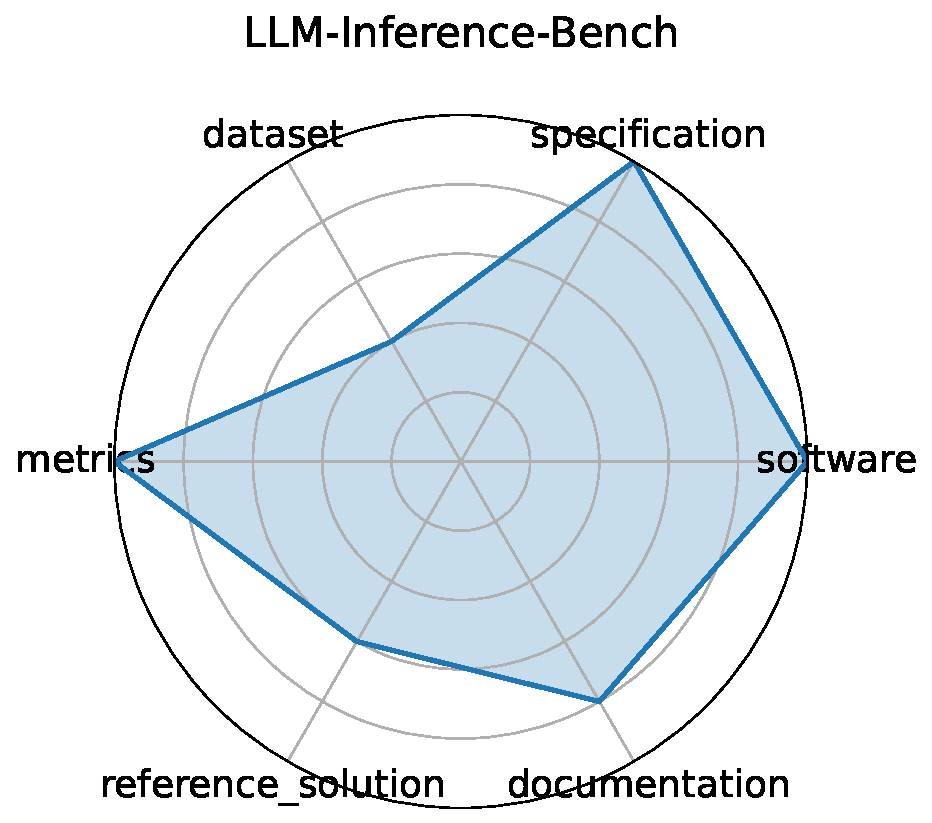
\includegraphics[width=0.2\textwidth]{llm-inference-bench_radar.pdf}
}}
\clearpage